% This file was created with tikzplotlib v0.9.12.
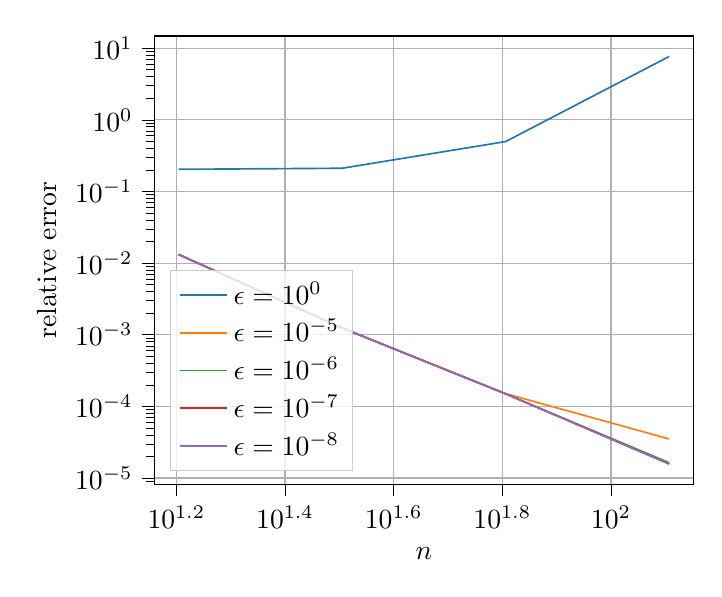
\begin{tikzpicture}

\definecolor{color0}{rgb}{0.12156862745098,0.466666666666667,0.705882352941177}
\definecolor{color1}{rgb}{1,0.498039215686275,0.0549019607843137}
\definecolor{color2}{rgb}{0.172549019607843,0.627450980392157,0.172549019607843}
\definecolor{color3}{rgb}{0.83921568627451,0.152941176470588,0.156862745098039}
\definecolor{color4}{rgb}{0.580392156862745,0.403921568627451,0.741176470588235}

\begin{axis}[
legend cell align={left},
legend style={
  fill opacity=0.8,
  draw opacity=1,
  text opacity=1,
  at={(0.03,0.03)},
  anchor=south west,
  draw=white!80!black
},
log basis x={10},
log basis y={10},
tick align=outside,
tick pos=left,
x grid style={white!69.0196078431373!black},
xlabel={\(\displaystyle n\)},
xmajorgrids,
xmin=14.4200074017733, xmax=142.024892424684,
xmode=log,
xtick style={color=black},
y grid style={white!69.0196078431373!black},
ylabel={relative error},
ymajorgrids,
ymin=8.15504073727232e-06, ymax=14.7610240059648,
ymode=log,
ytick style={color=black}
]
\addplot [semithick, color0]
table {%
16 0.203668257732831
32 0.210744691194534
64 0.496946252503836
128 7.66789250604972
};
\addlegendentry{$\epsilon=10^{0}$}
\addplot [semithick, color1]
table {%
16 0.013195361542501
32 0.00124244689527106
64 0.000150526247944769
128 3.50867177315718e-05
};
\addlegendentry{$\epsilon=10^{-5}$}
\addplot [semithick, color2]
table {%
16 0.0131953518904314
32 0.00124259195849113
64 0.00014947002751523
128 1.63297532322446e-05
};
\addlegendentry{$\epsilon=10^{-6}$}
\addplot [semithick, color3]
table {%
16 0.0131953408110014
32 0.00124257561862992
64 0.000149448212608262
128 1.56988053754698e-05
};
\addlegendentry{$\epsilon=10^{-7}$}
\addplot [semithick, color4]
table {%
16 0.0131953411695792
32 0.00124257578882137
64 0.000149450965997621
128 1.57030874951245e-05
};
\addlegendentry{$\epsilon=10^{-8}$}
\end{axis}

\end{tikzpicture}
